\documentclass{article}
\usepackage{fancyhdr}
\usepackage{extramarks}
\usepackage{amsmath}
\usepackage{amsthm}
\usepackage{amsfonts}
\usepackage{tikz}
\usepackage[plain]{algorithm}
\usepackage{algpseudocode}
\usepackage{enumerate}
\usepackage{amssymb}
\usepackage{multicol,multirow,array,listings,tabularx,lastpage,textcomp,booktabs}
\usetikzlibrary{automata,positioning,arrows}

%
% Basic Document Settings
%

\topmargin=-0.45in
\evensidemargin=0in
\oddsidemargin=0in
\textwidth=6.5in
\textheight=9.0in
\headsep=0.25in

\linespread{1.1}

\pagestyle{fancy}
\lhead{\hmwkAuthorName}
\chead{\hmwkClass:\ \hmwkTitle}
\rhead{\firstxmark}
\lfoot{\lastxmark}
\cfoot{\thepage}

\renewcommand\headrulewidth{0.4pt}
\renewcommand\footrulewidth{0.4pt}

\setlength\parindent{0pt}
\setlength{\parskip}{5pt}

%
% Create Problem Sections
%

\newcommand{\enterProblemHeader}[1]{
    \nobreak\extramarks{}{Problem \arabic{#1} continued on next page\ldots}\nobreak{}
    \nobreak\extramarks{Problem \arabic{#1} (continued)}{Problem \arabic{#1} continued on next page\ldots}\nobreak{}
}

\newcommand{\exitProblemHeader}[1]{
    \nobreak\extramarks{Problem \arabic{#1} (continued)}{Problem \arabic{#1} continued on next page\ldots}\nobreak{}
    \stepcounter{#1}
    \nobreak\extramarks{Problem \arabic{#1}}{}\nobreak{}
}

\setcounter{secnumdepth}{0}
\newcounter{partCounter}
\newcounter{homeworkProblemCounter}
\setcounter{homeworkProblemCounter}{1}
\nobreak\extramarks{Problem \arabic{homeworkProblemCounter}}{}\nobreak{}

%
% Homework Problem Environment
%
% This environment takes an optional argument. When given, it will adjust the
% problem counter. This is useful for when the problems given for your
% assignment aren't sequential. See the last 3 problems of this template for an
% example.
%
\newenvironment{homeworkProblem}[1][-1]{
    \ifnum#1>0
        \setcounter{homeworkProblemCounter}{#1}
    \fi
    \section{Problem \arabic{homeworkProblemCounter}}
    \setcounter{partCounter}{1}
    \enterProblemHeader{homeworkProblemCounter}
}{
    \exitProblemHeader{homeworkProblemCounter}
}

\newcommand\abs[1]{\lvert~#1~\rvert}
\newcommand{\st}{\mid}

\newcommand{\cmark}{\ding{51}}
\newcommand{\xmark}{\ding{55}}
 
\newcommand{\SUBSTRING}{\textsc{Substring}}
\newcommand{\REP}{\textsc{Rep}}
\newcommand{\blank}{\scalebox{1.5}{\square}}

%
% Homework Details
%   - Title
%   - Due date
%   - Class
%   - Section/Time
%   - Instructor
%   - Author
%

\newcommand{\hmwkTitle}{Homework\ \#3}
\newcommand{\hmwkDueDate}{Feb 15, 2024}
\newcommand{\hmwkClass}{CSE 105}
\newcommand{\hmwkClassInstructor}{Professor Minnes}
\newcommand{\hmwkAuthorName}{\textbf{Ray Tsai}}
\newcommand{\hmwkPID}{A16848188}

\newcommand{\gradeCorrect}{({\it Graded for correctness}) }
\newcommand{\gradeCorrectFirst}{\gradeCorrect\footnote{This means your solution 
will be evaluated not only on the correctness of your answers, but on your ability
to present your ideas clearly and logically. You should explain how you 
arrived at your conclusions, using
mathematically sound reasoning. Whether you use formal proof techniques or 
write a more informal argument
for why something is true, your answers should always be well-supported. 
Your goal should be to convince the
reader that your results and methods are sound.} }
\newcommand{\gradeComplete}{({\it Graded for completeness}) }
\newcommand{\gradeCompleteFirst}{\gradeComplete\footnote{This means you will 
get full credit so long as your submission demonstrates honest effort to 
answer the question. You will not be penalized for incorrect answers. 
To demonstrate your honest effort in answering the question, we 
expect you to include your attempt to answer *each* part of the question. 
If you get stuck with your attempt, you can still demonstrate 
your effort by explaining where you got stuck and what 
you did to try to get unstuck.} }

%
% Title Page
%

\title{
    \vspace{2in}
    \textmd{\textbf{\hmwkClass:\ \hmwkTitle}}\\
    \normalsize\vspace{0.1in}\small{Due\ on\ \hmwkDueDate\ at 23:59pm}\\
    \vspace{0.1in}\large{\textit{\hmwkClassInstructor}} \\
    \vspace{3in}
}

\author{
  \hmwkAuthorName \\
  \vspace{0.1in}\small\hmwkPID
}
\date{}

\renewcommand{\part}[1]{\textbf{\large Part \Alph{partCounter}}\stepcounter{partCounter}\\}

%
% Various Helper Commands
%

% Useful for algorithms
\newcommand{\alg}[1]{\textsc{\bfseries \footnotesize #1}}

% For derivatives
\newcommand{\deriv}[1]{\frac{\mathrm{d}}{\mathrm{d}x} (#1)}

% For partial derivatives
\newcommand{\pderiv}[2]{\frac{\partial}{\partial #1} (#2)}

% Integral dx
\newcommand{\dx}{\mathrm{d}x}

% Probability commands: Expectation, Variance, Covariance, Bias
\newcommand{\Var}{\mathrm{Var}}
\newcommand{\Cov}{\mathrm{Cov}}
\newcommand{\Bias}{\mathrm{Bias}}
\newcommand*{\Z}{\mathbb{Z}}
\newcommand*{\Q}{\mathbb{Q}}
\newcommand*{\R}{\mathbb{R}}
\newcommand*{\C}{\mathbb{C}}
\newcommand*{\N}{\mathbb{N}}
\newcommand*{\prob}{\mathds{P}}
\newcommand*{\E}{\mathds{E}}

\begin{document}

\maketitle

\pagebreak

\begin{homeworkProblem}
  Consider the push-down automata $M_1$ and $M_2$ over $\{a,b\}$ with stack alphabet $\{a, b\}$ whose state diagrams are

  \begin{center}
  \begin{multicols}{2}
    State diagram for $M_1$

    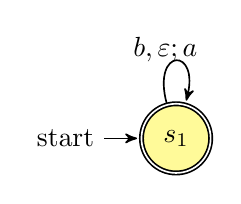
\begin{tikzpicture}[->,>=stealth',shorten >=1pt, auto, node distance=2cm, semithick]
    \tikzstyle{every state}=[text=black, fill=yellow!40]
    
    \node[initial,state, accepting] (s1)          {$s_1$};

    \path (s1) edge  [loop above, near start] node {$b,\varepsilon; a$} (s1) ;
    \end{tikzpicture}

    \columnbreak 

    State diagram for $M_2$

    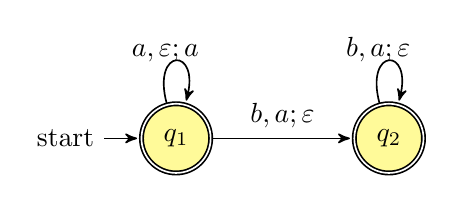
\begin{tikzpicture}[->,>=stealth',shorten >=1pt, auto, node distance=2cm, semithick]
    \tikzstyle{every state}=[text=black, fill=yellow!40]
    
    \node[initial,state, accepting] (q1)          {$q_1$}; \node[state, accepting]         (q2) [right of=q1, xshift=20pt] {$q_2$};
    
    \path (q1) edge  [loop above, near start] node {$a,\varepsilon; a$} (q1) (q1) edge [bend left=0] node {$b,a;\varepsilon$} (q2) (q2) edge [loop above, near start] node {$b,a;\varepsilon$} (q2) ;
    \end{tikzpicture}
  \end{multicols}
  \end{center}
  \begin{enumerate}[(a)]
    \item \gradeComplete What is the language $A_1$ recognized by $M_1$ and what is the language $A_2$ recognized by $M_2$? Include a sample string that is accepted and one that is rejected for each of these PDA. Justify these examples with sample accepting computations or with an explanation why there is no accepting computation.
    \begin{proof}
      Since $M_1$ only contains a state with a loop which only takes $b$ as an input, $A_1 = b^*$. Hence, $\varepsilon \in A_1$ and $a \notin A_1$, as the starting state is also an accepting state and there are simply no arrows for $a$'s to follow.
      
      For $M_2$ to take $b$ as an input, there has to be at least one $a$ in the memory stack, and thus the $b$'s in the string cannot precede $a$'s and the number of $b$ is at most that of $a$. Hence, $A_2 = \{a^mb^n \mid m \geq n, m, n \in \Z_{\geq 0}\}$. For instance, $\varepsilon \in A_2$ and $b \notin A_2$. $\varepsilon$ is obviously accepted as the starting state is also an accepting state. $b$ is rejected as there are no $a$'s in the memory stack for the $b$ to be sent to $q_2$.
    \end{proof}
    \item \gradeCorrect Design CFGs $G_1$ and $G_2$ over $\{a,b\}$ so that $L(G_1) = A_1$ and $L(G_2) = A_2$. A complete solution will include precise definitions for each of the parameters required to specify a CFG, as well as a brief explanation about why each string in $A_i$ can be derived in $G_i$ and each string not in $A_i$ cannot be derived in $G_i$ (for $i=1,2$).
    \begin{proof}
      Let $\Sigma = \{a, b\}$. Consider
      \[
        G_1 = (\{S_1\}, \Sigma, \{S_1 \to bS_1 \mid \varepsilon\}, S_1) \quad \text{and} \quad G_2 = (\{S_2\}, \Sigma, \{S_2 \to aS_2 \mid aS_2b \mid \varepsilon\}, S_2).
      \]
      Since $G_1$ repeatedly generates $b$ and terminates with $\varepsilon$, $L(G_1)$ contains $A_1$, the language of all strings that doesn't contain $a$. Let $s \notin A_1$. $s$ contains $A$. Since $G_1$ does not generate $a$, $a \notin L(G_1)$. Hence, $L(G_1) = A_1$. 

      Let $k \in A_2$. $k$ is of the form $a^mb^n$, for $m \geq n \geq 0$. Note that whenever $G_2$ generates $b$, it generates an $a$ preceding the $b$, but the generation of $a$ is not binded to $b$. Hence, $k$ is obviously in $L(G_2)$. Let $p \notin A_2$. $p$ either has a $b$ preceding $a$ or has more $b$ than $a$, both of which contradicts the rules defined for $G_2$, and thus $p \notin L(G_2)$.
    \end{proof}
    \item \gradeComplete Remember that the definition of set-wise concatenation is: for languages $L_1, L_2$ over the alphabet $\Sigma$, we have the associated set of strings
    \[
        L_1 \circ L_2 = \{ w \in \Sigma^* ~|~ w = uv \text{ for some strings } u \in L_1 \text{ and } v \in L_2 \}
    \]
    In class (and in the review quiz) we learned that the class of context-free languages is closed under set-wise concatenation. The proof of this closure claim using CFGs uses the construction: given $G_1 = ( V_1, \Sigma, R_1, S_1)$ and $G_2 = (V_2, \Sigma, R_2, S_2)$ with $V_1 \cap V_2 = \emptyset$ and $S_{new} \notin V_1 \cup V_2$, define a new CFG
    $$G = (V_1 \cup V_2 \cup \{S_{new}\}, \Sigma, R_1 \cup R_2 \cup \{S_{new} \to S_1 S_2\}, S_{new})$$ Apply this construction to your grammars from part (b) and give a sample derivation of a string in $A_1 \circ A_2$ in this resulting grammar.
    \begin{proof}
      Applying this construction to $G_1, G_2$, we get
      \[
        G = (\{S_1, S_2, S_{new}\}, \Sigma, R, S_{new}),
      \]
      where the set of rules $R$ is 
      \begin{gather*}
        S_{new} \to S_1S_2 \\
        S_1 \to bS_1 \mid \varepsilon \\
        S_2 \to aS_2 \mid aS_2b \mid \varepsilon.
      \end{gather*}
      An example of derivation of $\varepsilon \in A_1 \circ A_2$ is
      \[
        S_{new} \Rightarrow S_1S_2 \Rightarrow \varepsilon S_2 \Rightarrow \varepsilon.
      \]
    \end{proof}
    \item \gradeCorrect If we try to extrapolate the construction that we used to prove that the class of regular languages is closed under set-wise concategation, we would get the following construction for PDAs: Given $M_1 = (Q_1, \Sigma, \Gamma_1, \delta_1, q_1, F_1)$ and $M_2 = (Q_2, \Sigma, \Gamma_2, \delta_2, q_2, F_2)$ with $Q_1 \cap Q_2 = \emptyset$, define $Q = Q_1 \cup Q_2$, $\Gamma = \Gamma_1 \cup \Gamma_2$, and
    $$M = (Q, \Sigma, \Gamma, \delta, q_1, F_2)$$ with $\delta: Q \times \Sigma_\varepsilon \times \Gamma_\varepsilon \to \mathcal{P}(Q \times \Gamma_\varepsilon)$ given by 
    $$\delta( q,a,b) = \begin{cases} \delta_1 (q,a,b) &\text{if $q \in Q_1 \setminus F_1$, $a \in \Sigma_\varepsilon$, $b \in {\Gamma_1}_\varepsilon$} \\
        \delta_2 (q,a,b) &\text{if $q \in Q_2$, $a \in \Sigma_\varepsilon$, $b \in {\Gamma_2}_\varepsilon$} \\
        \delta_1 (q,a,b) &\text{if $q \in F_1$, $a \in \Sigma$ or $b\in \Gamma_1$}\\
        \delta_1 (q,a,b) \cup \{ (q_2, \varepsilon)\} &\text{if $q \in F_1$, $a =\varepsilon$, $b=\varepsilon$}\\
        \emptyset &\text{otherwise} \end{cases}$$ Apply this construction to the machines $M_1$ and $M_2$ from part (a), and then use the resulting PDA to prove that {\it this} construction cannot be used to prove that the class of context-free languages is closed under set-wise concatenation. A complete solution will include (1) the state diagram of the machine $M$ that results from applying this construction to $M_1$ and $M_2$, (2) an example of a string that is accepted by this PDA $M$ but that is {\bf not} in the language $A_1 \circ A_2$ with a description of the computation that witnesses that this string is accepted by $M$ and an explanation of why this string is not in $A_1 \circ A_2$ by referring back to the definitions of $A_1$, $A_2$, and set-wise concatenation.
    \begin{proof}
      The following is the state diagram for $M$:
      \begin{center}
        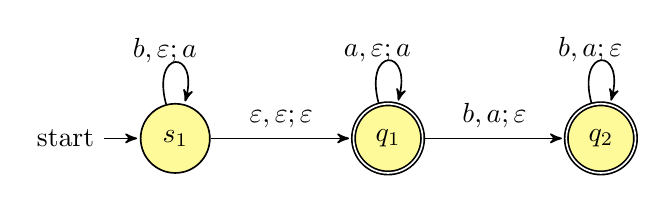
\begin{tikzpicture}[->,>=stealth',shorten >=1pt, auto, node distance=2cm, semithick]
          \tikzstyle{every state}=[text=black, fill=yellow!40]
          
          \node[initial,state] (s1) {$s_1$}; \node[state, accepting] (q1) [right of=s1, xshift=20pt] {$q_1$}; \node[state, accepting]  (q2) [right of=q1, xshift=20pt] {$q_2$};
          
          \path (s1) edge  [] node {$\varepsilon,\varepsilon; \varepsilon$} (q1) (s1) edge  [loop above, near start] node {$b,\varepsilon; a$} (s1) (q1) edge  [loop above, near start] node {$a,\varepsilon; a$} (q1) (q1) edge [bend left=0] node {$b,a;\varepsilon$} (q2) (q2) edge [loop above, near start] node {$b,a;\varepsilon$} (q2) ;
        \end{tikzpicture}
      \end{center}
      Consider the string $s = babb$. $babb$ is accepted by $M$, following the path $s_1 \to q_1 \to q_2 \to q_2$. Note that $s$ is allowed to go through $q_2$ twice, as the prefix $ba$ pushes two $a$'s onto the memory stack priorly. However, $s$ is not a valid concatenation of $A_1$ and $A_2$, as $babb \notin A_1$ and none of $babb, abb, bb, b$ are in $A_2$. 
    \end{proof}
  \end{enumerate}
\end{homeworkProblem}

\newpage

\begin{homeworkProblem}
  Informally, we think of regular languages as potentially simpler than context-free languages. In this question, you'll make this precise by showing that every regular language is context-free, in two ways.
  \begin{enumerate}[(a)]
  \item\gradeCorrect When we first introduced PDAs we saw that any NFA can be transformed to a PDA by not using the stack of the PDA at all. Make this precise by completing the following construction: Given a NFA $N = (Q, \Sigma, \delta_N, q_0, F)$ we define a PDA $M$ with $L(M) = L(N)$ by choosing \ldots A complete solution will have precise, correct definitions for each of the defining parameters of $M$: the set of states, the input alphabet, the stack alphabet, the transition function, the start state, and the set of accept states. Be careful to use notation that matches the types of the objects involved.

  \begin{proof}
    $M = (Q, \Sigma, \emptyset, \delta_M, q_0, F)$, where $\delta_M \colon Q \times \Sigma_{\varepsilon} \times \emptyset_{\varepsilon} \to \mathcal{P}(Q \times \emptyset_{\varepsilon})$ sends $(q, \sigma, \gamma)$ to $\delta_N(q, \sigma) \times \{\varepsilon\}$.
  \end{proof}

  \item\gradeCorrect In the book on page 107, the top paragraph describes a procedure for converting DFA to CFGs:
  \begin{quote}
    You can convert any DFA into an equivalent CFG as follows. Make a variable $R_i$ for each state $q_i$ of the DFA. Add the rule $R_i \to aR_j$ to the CFG if $\delta(q_i,a) =q_j$ is a transition in the DFA. Add the rule $R_i\to \varepsilon$ if $q_i$ is an accept state of the DFA. Make $R_0$ the start variable ofthe grammar, where $q_0$ is the start state of the machine. Verify on your own that the resulting CFG generates the same language that the DFA recognizes.
  \end{quote}

  Use this construction to get a context-free grammar generating the language 
  \[
      \{ w \in \{0,1\}^* \mid w \text{ does not have $11$ as a substring}\}
  \]
  by (1) designing a DFA that recognizes this language and then (2) applying the construction from the book to convert the DFA to an equivalent CFG. A complete submission will include the state diagram of the DFA, a brief justification of why it recognizes the language, and then the complete and precise definition of the CFG that results from applying the construction from the book to this DFA. {\it Ungraded bonus: take a sample string in the language and see how the computation of the DFA on this string translates to a derivation in your grammar.}

  \begin{proof}
    Consider the following state diagram of a DFA $M$:
    \begin{center}
      \begin{tikzpicture}[->,>=stealth',shorten >=1pt, auto, node distance=2cm, semithick]
        \tikzstyle{every state}=[text=black, fill=yellow!40]
        
        \node[initial,state, accepting] (q0) {$q_0$}; \node[state, accepting] (q1) [right of=s1, xshift=20pt] {$q_1$}; \node[state]  (gulag) [right of=q1, xshift=20pt] {\tiny gulag};
        
        \path (q0) edge  [bend left=20] node {$1$} (q1) (q0) edge  [loop above] node {$0$} (q0) (q1) edge  [bend left=20] node {$0$} (q0) (q1) edge [] node {$1$} (gulag) (gulag) edge [loop above] node {$0, 1$} (gulag) ;
      \end{tikzpicture}
    \end{center}
    Call that language $S$. Note that the states $q_0$ and $q_1$ record the previous input character. Suppose $s \in S$. Since $s$ does not contain consecutive $1$'s, $s$ would never get sent from $q_1$ to the gulag, and thus $s \in L(M)$. Suppose $s \notin S$. Then, $s$ contains consecutive $1$'s, and so it would eventually get sent to the gulag. Hence, $L(M) = S$. Applying the construction to $M$, we get a CFG $G = (\{R_0, R_1, R_{gulag}\}, \{0, 1\}, R, R_0)$, where the set of rules $R$ is
    \begin{gather*}
      R_0 \to 0R_0 \mid 1R_1 \mid \varepsilon \\
      R_1 \to 0R_0 \mid 1R_{gulag} \mid \varepsilon \\
      R_{gulag} \to 0R_{gulag} \mid 1R_{gulag}.
    \end{gather*}
  \end{proof}
\end{enumerate}
\end{homeworkProblem}

\newpage

\begin{homeworkProblem}
  On page 4 of the week 4 notes, we have the following list of languages over the alphabet $\{a,b\}$

  \begin{center}
  \begin{tabular}{ccc}
    $\{a^nb^n \mid 0  \leq n  \leq 5 \}$ &$\{b^n a^n \mid  n  \geq 2\}$ &$\{a^m b^n \mid  0 \leq m\leq n\}$
  \end{tabular}
  \begin{tabular}{cc}
    $\{a^m b^n \mid  m \geq n+3,  n \geq 0\}$ &$\{b^m a^n \mid  m \geq 1, n \geq  3\}$\\
    $\{ w  \in \{a,b\}^* \mid w = w^\mathcal{R} \}$ &$\{ ww^\mathcal{R} \mid w\in \{a,b\}^* \}$ \\
  \end{tabular}
  \end{center}
  \begin{enumerate}[(a)]
    \item\gradeComplete Pick one of the regular languages and design a regular expression that describes it. Briefly justify your regular expression by connecting the subexpressions of it to the intended language and referencing relevant definitions.
    \begin{proof}
      Consider $S = \{a^nb^n \mid 0  \leq n  \leq 5 \}$. $\varepsilon \cup ab \cup aabb \cup aaabbb \cup aaaabbbb \cup aaaaabbbbb$ describes $S$, as it is the union of all strings in $S$.
    \end{proof}
    \item\gradeComplete Pick another one of the regular languages and design a DFA that recognizes it. Draw the state diagram of your DFA. Briefly justify your design by explaining the role each state plays in the machine, as well as a brief justification about how the strings accepted and rejected by the machine connect to the specified language.
    \begin{proof}
      Consider the following DFA $M$ that recognizes $T = \{b^m a^n \mid  m \geq 1, n \geq 3\}$:
      \begin{center}
        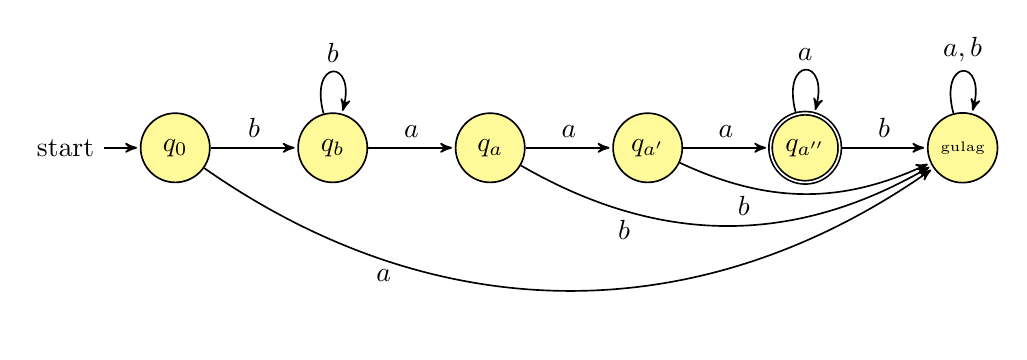
\begin{tikzpicture}[->,>=stealth',shorten >=1pt, auto, node distance=2cm, semithick]
          \tikzstyle{every state}=[text=black, fill=yellow!40]
          
          \node[initial,state] (q0) {$q_0$}; \node[state] (qb) [right of=q0, xshift=0pt] {$q_b$}; \node[state] (qa) [right of=qb, xshift=0pt] {$q_a$}; \node[state] (qa2) [right of=qa, xshift=0pt] {$q_{a'}$}; \node[state, accepting] (qa3) [right of=qa2, xshift=0pt] {$q_{a''}$}; \node[state]  (gulag) [right of=qa3, yshift=0pt] {\tiny gulag};
          
          \path (q0) edge  [bend left=0] node {$b$} (qb) (qb) edge [loop above] node {$b$} (qb) (qa) edge [] node {$a$} (qa2) (qa2) edge [] node {$a$} (qa3) (qb) edge [] node {$a$} (qa) (q0) edge [bend right=35, below, near start] node {$a$} (gulag) (qa) edge [bend right=30, below, near start] node {$b$} (gulag) (qa2) edge [bend right=25, below, near start] node {$b$} (gulag) (qa3) edge [] node {$b$} (gulag) (gulag) edge [loop above] node {$a, b$} (gulag) (qa3) edge [loop above] node {$a$} (qa3) ;
        \end{tikzpicture}
      \end{center}
      The states count the number of times we have met both $a$ and $b$, to ensure the input strings are of the form $bb\dots baa\dots a$ and have at least $1$ $b$ and 3 $a$'s. 
    \end{proof}
    \item\gradeComplete Pick one of the nonregular languages and design a PDA that recognizes it. Draw the state diagram of your PDA. Briefly justify your design by explaining the role each state plays in the machine, as well as a brief justification about how the strings accepted and rejected by the machine connect to the specified language.
    \begin{proof}
      Consider the set $X = \{a^m b^n \mid  0 \leq m\leq n\}$. The following PDA recognizes $X$:
      \begin{center}
        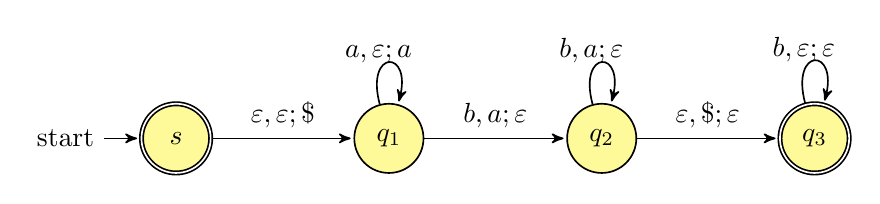
\begin{tikzpicture}[->,>=stealth',shorten >=1pt, auto, node distance=2cm, semithick]
          \tikzstyle{every state}=[text=black, fill=yellow!40]
          
          \node[initial,state, accepting] (s)          {$s$}; \node[state] (q1) [right of=s, xshift=20pt]        {$q_1$}; \node[state]         (q2) [right of=q1, xshift=20pt] {$q_2$}; \node[state, accepting]         (q3) [right of=q2, xshift=20pt] {$q_3$};
          
          \path (s) edge [bend left=0] node {$\varepsilon,\varepsilon; \$ $} (q1) (q1) edge  [loop above, near start] node {$a,\varepsilon; a$} (q1) (q1) edge [bend left=0] node {$b,a;\varepsilon$} (q2) (q2) edge [loop above, near start] node {$b,a;\varepsilon$} (q2) (q2) edge [bend left=0] node {$\varepsilon,\$;\varepsilon$} (q3) (q3) edge [loop above, near start] node {$b,\varepsilon;\varepsilon$} (q3) ;
          \end{tikzpicture}
      \end{center}
      The PDA stores the number of $a$'s in the prefix on the memory stack, and ensures the strings have enough $b$'s to deplete the stack before reaching the accepting state $q_3$. Hence, $X$ is recognized by the PDA above.
    \end{proof}
    \item\gradeComplete Pick one of the nonregular languages and write a CFG that generates it. Briefly justify your design by by demonstrating how derivations in the grammar relate to the intended language.
    \begin{proof}
      Consider $Y = \{ ww^\mathcal{R} \mid w\in \{a,b\}^* \}$. The CFG $G = (\{S\}, \{a, b\}, \{S \to aSa \mid bSb \mid \varepsilon\}, S)$ generates $Y$. Since every rule in $R$ produces the same elements on both sides of $S$, $G$ inductively generates symmtric strings over $\{a, b\}$, and this is exactly what $Y$ is.
    \end{proof}
  \end{enumerate}
\end{homeworkProblem}

\newpage

\begin{homeworkProblem}
  Consider the Turing machine $T$ over the input alphabet $\Sigma = \{0,1\}$ with  the state diagram below (the tape alphabet is $\Gamma = \{ 0,1,X,\square\}$). Convention: we do not include the node for the reject state $q_{rej}$ and any missing transitions in the state diagram have value $(q_{rej},\square,R)$
  \begin{center}
  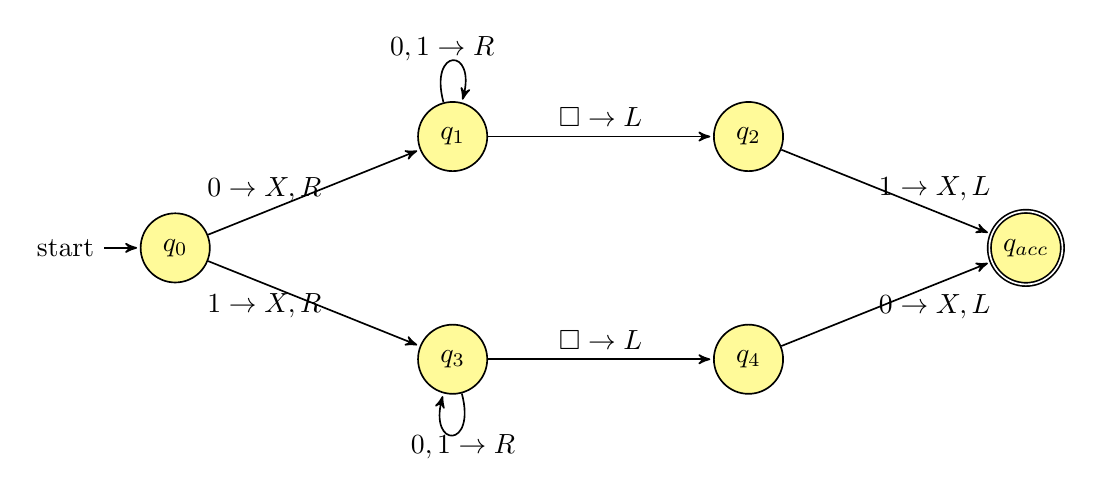
\begin{tikzpicture}[->,>=stealth',shorten >=1pt, auto, node distance=2cm, semithick]
    \tikzstyle{every state}=[text=black, fill=yellow!40]
    
    \node[initial,state] (q0)          {$q_0$}; \node[state] (q1)  [above right of=q0, xshift=60pt] {$q_{1}$}; \node[state] (q2)  [right of=q1, xshift=50pt] {$q_{2}$}; \node[state] (q3)  [below right of=q0, xshift=60pt] {$q_{3}$}; \node[state] (q4)  [right of=q3, xshift=50pt] {$q_{4}$}; \node[state, accepting]         (qacc) [below right of=q2, xshift=60pt] {$q_{acc}$};
    
    \path (q1) edge  [loop above, near start] node {$0,1 \to R$} (q1) (q3) edge  [loop below, near start] node {$0,1 \to R$} (q3) (q0) edge [bend left=0, above, near start] node {$0\to X, R$} (q1) (q0) edge [bend left=0, below, near start] node {$1\to X, R$} (q3) (q1) edge [bend left=0] node {$\square \to L$} (q2) (q2) edge [bend left=0, above, near end] node {$1\to X, L$} (qacc) (q3) edge [bend left=0] node {$\square \to L$} (q4) (q4) edge [bend left=0, below, near end] node {$0\to X, L$} (qacc) ;
    \end{tikzpicture}
  \end{center}

  \begin{enumerate}[(a)]
    \item\gradeCorrect Specify an example string $w_1$ of length $4$ over $\Sigma$ that is {\bf accepted} by this Turing machine, or explain why there is no such example. A complete solution will include either (1) a precise and clear description of your example  string and a precise and clear description of the accepting computation of the Turing machine on this string or (2) a sufficiently general and correct argument why there is no such example, referring back to the relevant definitions.
    
    To describe a computation of a Turing machine, include the contents of the tape, the state of the machine, and the location of the read/write head at each step in the computation.
    
    {\it Hint:} In class we've drawn pictures to represent the configuration of the machine at each step in a computation.  You may do so or you may choose to describe these configurations in words.

    \begin{proof}
      Consider $w_1 = 0001$. The following is the computation of $w_1$ in $T$:
      \begin{center}
        \begin{tabular}{|c|c|c|c|c|}
          \hline
          \multicolumn{1}{|c}{$q_0\downarrow$} &  \multicolumn{4}{c|}{\phantom{A}}\\
          \hline
          $0$ & $0$  & $0$ & $1$& $\square $\\
          \hline
          \multicolumn{1}{|c}{\phantom{A}} & \multicolumn{1}{c}{$q_1\downarrow$} & \multicolumn{3}{c|}{\phantom{A}}\\
          \hline
          $X$ & $0$  & $0$ & $1$& $\square $\\
          \hline
          \multicolumn{2}{|c}{\phantom{A}} & \multicolumn{1}{c}{$q_1\downarrow$} & \multicolumn{2}{c|}{\phantom{A}}\\
          \hline
          $X$ & $0$  & $0$ & $1$& $\square $\\          
          \hline
          \multicolumn{3}{|c}{\phantom{A}} & \multicolumn{1}{c}{$q_1\downarrow$} & \multicolumn{1}{c|}{\phantom{A}}\\          
          \hline
          $X$ & $0$  & $0$ & $1$& $\square $\\          
          \hline
          \multicolumn{4}{|c}{\phantom{A}} & \multicolumn{1}{c|}{$q_1\downarrow$}\\          
          \hline
          $X$ & $0$  & $0$ & $1$& $\square $\\         
          \hline
          \multicolumn{3}{|c}{\phantom{A}} & \multicolumn{1}{c}{$q_2\downarrow$} & \multicolumn{1}{c|}{\phantom{A}}\\          
          \hline
          $X$ & $0$  & $0$ & $1$& $\square $\\   
          \hline
          \multicolumn{2}{|c}{\phantom{A}} & \multicolumn{1}{c}{$q_{acc}\downarrow$} & \multicolumn{2}{c|}{\phantom{A}}\\          
          \hline
          $X$ & $0$  & $0$ & $X$& $\square $\\   
          \hline
          \end{tabular}
      \end{center}
      Therefore, $T$ accepts $w_1$.
    \end{proof}
    
    \item\gradeCorrect Specify an example string $w_2$ of length $3$ over $\Sigma$ that is {\bf rejected} by this Turing machine or explain why there is no such example. A complete solution will include either (1) a precise and clear description of your example  string and a precise and clear description of the rejecting computation of the Turing machine on this string or (2) a sufficiently general and correct argument why there is no such example, referring back to the relevant definitions.
    \begin{proof}
      Consider $w_2 = 000$. The following is the computation of $w_1$ in $T$:
      \begin{center}
        \begin{tabular}{|c|c|c|c|}
          \hline
          \multicolumn{1}{|c}{$q_0\downarrow$} &  \multicolumn{3}{c|}{\phantom{A}}\\
          \hline
          $0$ & $0$  & $0$ & $\square $ \\
          \hline
          \multicolumn{1}{|c}{\phantom{A}} & \multicolumn{1}{c}{$q_1\downarrow$} & \multicolumn{2}{c|}{\phantom{A}}\\
          \hline
          $X$ & $0$  & $0$ & $\square $ \\
          \hline
          \multicolumn{2}{|c}{\phantom{A}} & \multicolumn{1}{c}{$q_1\downarrow$} & \multicolumn{1}{c|}{\phantom{A}}\\
          \hline
          $X$ & $0$  & $0$ & $\square $ \\          
          \hline
          \multicolumn{3}{|c}{\phantom{A}} & \multicolumn{1}{c|}{$q_1\downarrow$}\\          
          \hline
          $X$ & $0$  & $0$ & $\square $ \\          
          \hline
          \multicolumn{2}{|c}{\phantom{A}} & \multicolumn{1}{c}{$q_2\downarrow$} & \multicolumn{1}{c|}{\phantom{A}}\\          \hline
          $X$ & $0$  & $0$ & $\square $ \\         
          \hline
          \multicolumn{3}{|c}{\phantom{A}} & \multicolumn{1}{c|}{$q_{rej}\downarrow$} \\          \hline
          $X$ & $0$  & $\square$ & $\square $ \\         
          \hline
          \end{tabular}
      \end{center}
      Therefore, $T$ rejects $w_2$.
    \end{proof}

    \item\gradeCorrect Specify an example string $w_3$ of length $2$ over $\Sigma$ on which  the computation of this Turing machine {\bf loops} or explain why there is no such example. A complete solution will include either (1) a precise and clear description of your example string and a precise and clear description of the looping (non-halting) computation of the Turing machine on this string or (2) a sufficiently general and correct argument why there is no such example, referring back to the relevant definitions.

    \begin{proof}
      Such $w_3$ does not exist. In the computation of $T$, $T$ keeps reading the next right element until it reads a blank. After $T$ reads a blank, $T$ proceeds to either $q_2$ or $q_4$. Since $w_3$ is of a finite length, $T$ will eventually read a blank, and thus it must reach either $q_2$ or $q_4$. However, $q_2$ and $q_4$ only points to either the accepting or rejecting state, and thus $T$ must halt if the input is a string of length 2.
    \end{proof}

    \item\gradeComplete Write an implementation level description of the Turing machine $T$.
    \begin{proof}
      $T$ starts in $q_0$ processes the input by marking visited symbols with an $X$ and moving the tape head to the right. If the first input characted $T$ reads is 0, then it transitions to $q_1$. Otherwise, if the first input character is 0, then it transitions to $q_3$. Afterwards, $T$ repeatedly reads the next right character until reading a $\square$, which indicates that the string has ended. It then transitions to $q_2/q_4$, prints a $\square$, and reads the left character, namely the last character of the string. If the ending character of the string is different from the starting character, then the machine transitions to the rejecting state. Otherwise, $T$ transitions to the accepting state. transitions to 
    \end{proof}
  \end{enumerate}
\end{homeworkProblem}
\end{document}